We perform the full \hww\ analysis using the \zm\ method for Drell-Yan estimation and we compare it with the default analysis (\routin\ method).
First, we compare the analysis components that are affected by the Drell-Yan estimation method 
(data/MC scale factors and shapes for the BDT analysis) and then we compare the expected limits resulting from the two analyses.

The scale factors from the two estimation methods, reported in Table~\ref{tab:scalefactors}, are compatible within the uncertainties.
However, especially in the 0-jet bin, the error can be larger than 50\% and a proper comparison is difficult.

The \routin-based analysis uses as central shape MC events in the region with 30$<$\met$<$37 \GeV and as alternative shapes the MC in the signal region (``up'')
 and its mirror shape with respect to central (``down'').
With the \zm\ method, the central shape can be naturally taken from data weighting the events in the fail region with the corresponding \zm\ value;
the shape variations are still provided by the signal region in MC.
A comparison of the shapes used in the \routin- and \zm-based analyses is shown in Figures~\ref{fig:zjets_shape_mh115}-\ref{fig:zjets_shape_mh140}.
Shapes from the \zm\ method are generally suffering more from statistical fluctuations, but, when the unceratinty is not too large, 
similar features to the \routin\ case can be observed. As an example, both in Fig.~\ref{subfig:routin_zjets_shape_mh130_1jet} and 
Fig.~\ref{subfig:zeta_zjets_shape_mh130_1jet} there is a sharp peak at 0.7 and a broad bump below 0.2.

Considering the same flavor final states only, the resulting expected limits are compatible  within 10\% with the deafult analysis and 
show almost no difference when combined with the opposite flavor (Figures~\ref{tab:sf_limits} and \ref{tab:sfof_limits}).

%%%%%
\begin{table}[!ht]
\begin{center}
\begin{tabular} {|c|cc|}
\hline
Analysis  & \routin\ method & \zm\ method \\
\hline 
\hline
\multicolumn{3}{|c|}{0-jet} \\
\hline 
 WW level & 3.05$\pm$1.75 & 4.34$\pm$1.82 \\
 \mHi=115 & 5.28$\pm$3.51 & 2.12$\pm$1.47 \\
 \mHi=120 & 5.66$\pm$3.75 & 2.43$\pm$1.46 \\
 \mHi=130 & 4.07$\pm$2.80 & 2.69$\pm$1.33 \\
 \mHi=140 & 3.57$\pm$2.46 & 2.57$\pm$1.17 \\
 \mHi=150 & 2.76$\pm$2.86 & 3.03$\pm$1.41 \\
 \mHi=160 & 1.53$\pm$2.73 & 2.22$\pm$2.01 \\
 \mHi=170 & 0.75$\pm$1.65 & 1.00$\pm$1.00 \\
 \mHi=180 & 0.33$\pm$0.78 & 1.00$\pm$1.00 \\
 \mHi=190 & 1.08$\pm$1.50 & 1.00$\pm$1.00 \\
 \mHi=200 & 1.25$\pm$1.02 & 1.00$\pm$1.00 \\
\hline 
\hline
\multicolumn{3}{|c|}{1-jet} \\
\hline 
 WW level & 2.39$\pm$0.45 & 2.86$\pm$0.88 \\
 \mHi=115 & 5.05$\pm$2.22 & 7.74$\pm$2.81 \\
 \mHi=120 & 5.46$\pm$2.35 & 6.87$\pm$2.33 \\
 \mHi=130 & 3.39$\pm$1.75 & 4.99$\pm$1.64 \\
 \mHi=140 & 4.50$\pm$2.29 & 5.46$\pm$1.77 \\
 \mHi=150 & 5.25$\pm$2.00 & 4.23$\pm$1.33 \\
 \mHi=160 & 7.33$\pm$3.03 & 4.51$\pm$1.54 \\
 \mHi=170 & 9.58$\pm$4.18 & 1.33$\pm$1.94 \\
 \mHi=180 & 7.76$\pm$3.35 & 4.45$\pm$2.72 \\
 \mHi=190 & 4.53$\pm$1.77 & 3.84$\pm$1.69 \\
 \mHi=200 & 4.46$\pm$1.48 & 3.91$\pm$1.71 \\
\hline 
\hline
\multicolumn{3}{|c|}{2-jet} \\
\hline 
 WW level & 3.11$\pm$0.62 & 2.00$\pm$0.62 \\
\hline 
\end{tabular}
\caption{Drell-Yan data/MC scale factors for \hww\ analysis using 2011 data. Unceratinties include both statistic and systematic errors.}
\label{tab:scalefactors}
\end{center}
\end{table}
%%%%%


%%%%%%%%
\begin{figure}[!hbtp]
\begin{center}
\subfigure[0-jet, \routin~method]{\label{subfig:routin_zjets_shape_mh115_0jet}
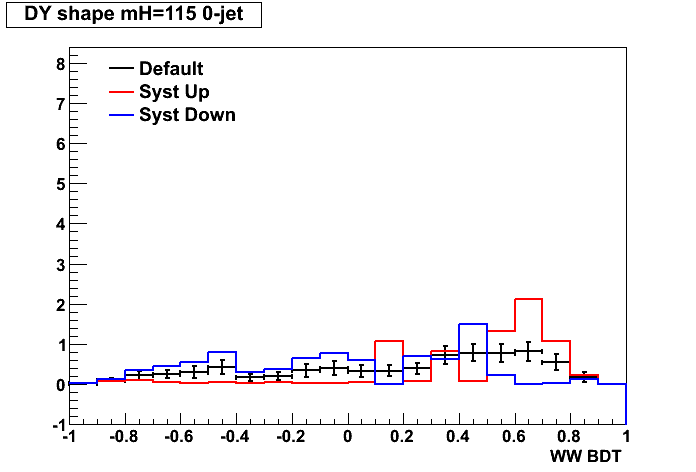
\includegraphics[width=.4\textwidth]{figures/dyshape_routin/zjets_shape_mh115_0jet.png}}
\subfigure[0-jet, \zm~method]{\label{subfig:zeta_zjets_shape_mh115_0jet}
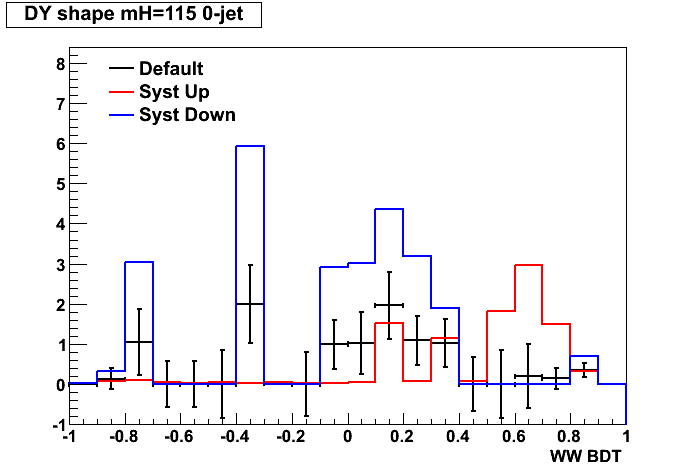
\includegraphics[width=.4\textwidth]{figures/dyshape_zeta/zjets_shape_mh115_0jet.png}}\\
\subfigure[1-jet, \routin~method]{\label{subfig:routin_zjets_shape_mh115_1jet}
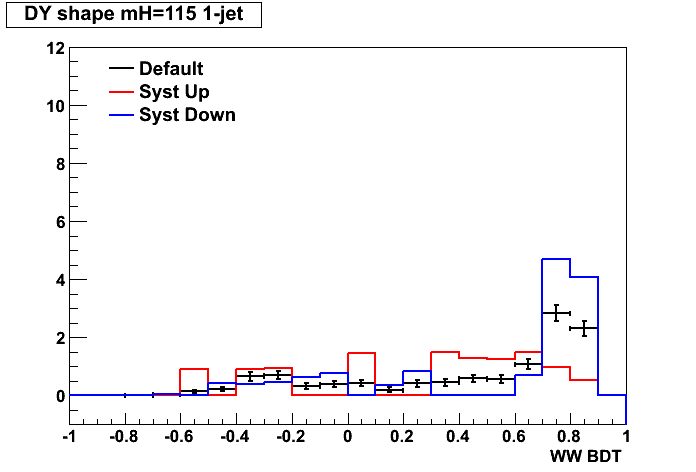
\includegraphics[width=.4\textwidth]{figures/dyshape_routin/zjets_shape_mh115_1jet.png}}
\subfigure[1-jet, \zm~method]{\label{subfig:zeta_zjets_shape_mh115_1jet}
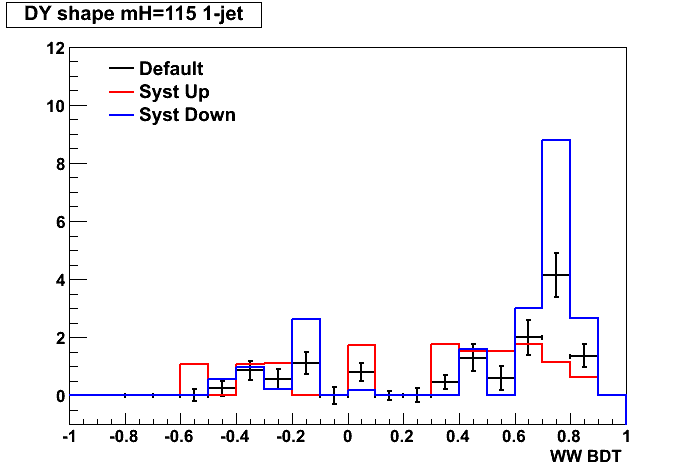
\includegraphics[width=.4\textwidth]{figures/dyshape_zeta/zjets_shape_mh115_1jet.png}}
\caption{\dyll~shape in \mHi=115 \GeVcc analysis.}
\label{fig:zjets_shape_mh115}
\end{center}
\end{figure}
%%%%%%%%

%%%%%%%%
\begin{figure}[!hbtp]
\begin{center}
\subfigure[0-jet, \routin~method]{\label{subfig:routin_zjets_shape_mh120_0jet}
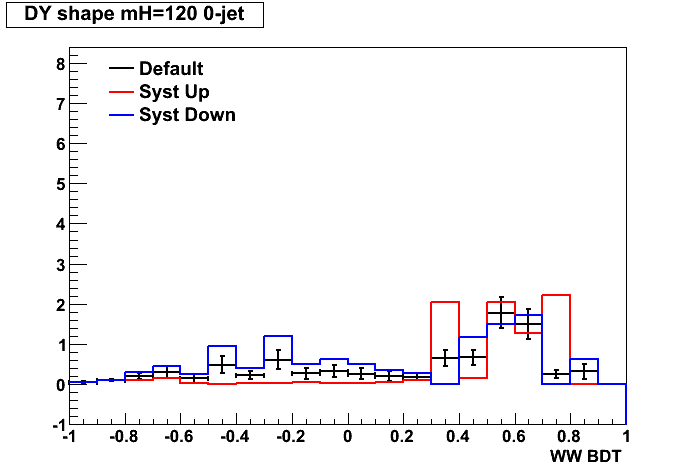
\includegraphics[width=.4\textwidth]{figures/dyshape_routin/zjets_shape_mh120_0jet.png}}
\subfigure[0-jet, \zm~method]{\label{subfig:zeta_zjets_shape_mh120_0jet}
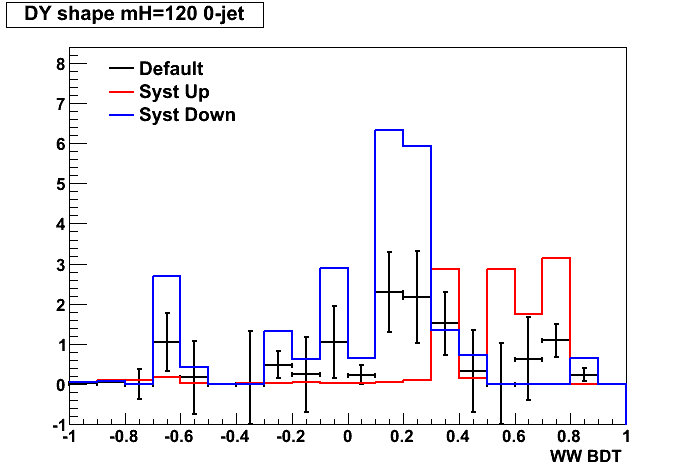
\includegraphics[width=.4\textwidth]{figures/dyshape_zeta/zjets_shape_mh120_0jet.png}}\\
\subfigure[1-jet, \routin~method]{\label{subfig:routin_zjets_shape_mh120_1jet}
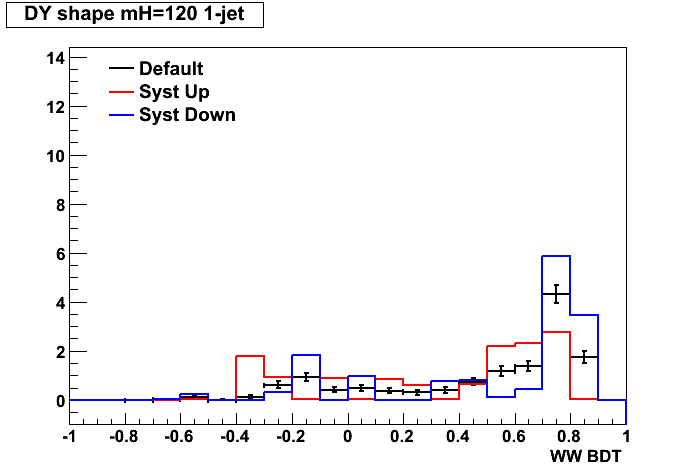
\includegraphics[width=.4\textwidth]{figures/dyshape_routin/zjets_shape_mh120_1jet.png}}
\subfigure[1-jet, \zm~method]{\label{subfig:zeta_zjets_shape_mh120_1jet}
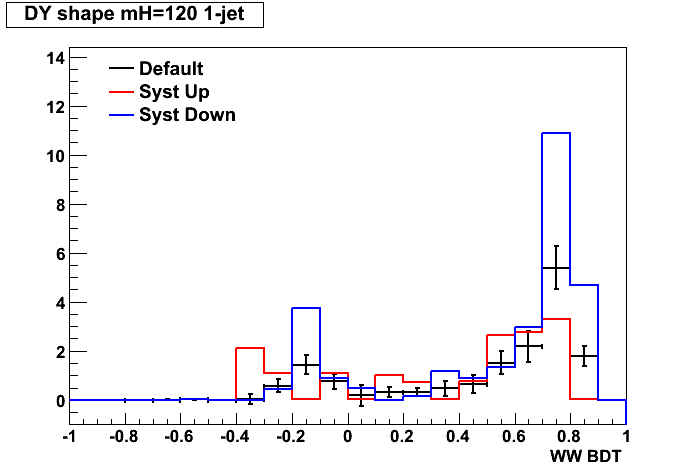
\includegraphics[width=.4\textwidth]{figures/dyshape_zeta/zjets_shape_mh120_1jet.png}}
\caption{\dyll~shape in \mHi=120 \GeVcc analysis.}
\label{fig:zjets_shape_mh120}
\end{center}
\end{figure}
%%%%%%%%

%%%%%%%%
\begin{figure}[!hbtp]
\begin{center}
\subfigure[0-jet, \routin~method]{\label{subfig:routin_zjets_shape_mh130_0jet}
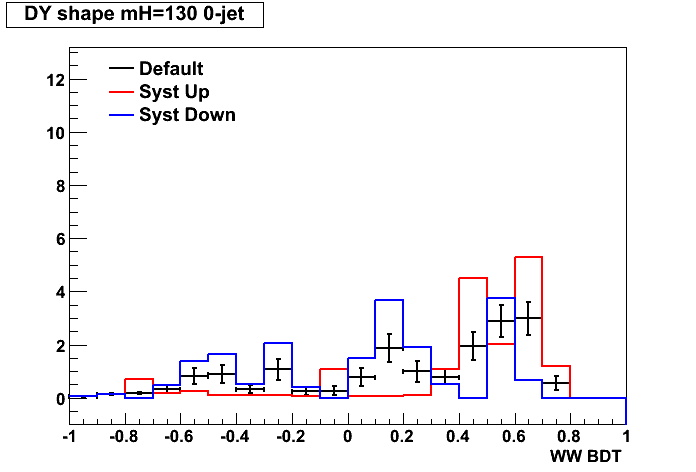
\includegraphics[width=.4\textwidth]{figures/dyshape_routin/zjets_shape_mh130_0jet.png}}
\subfigure[0-jet, \zm~method]{\label{subfig:zeta_zjets_shape_mh130_0jet}
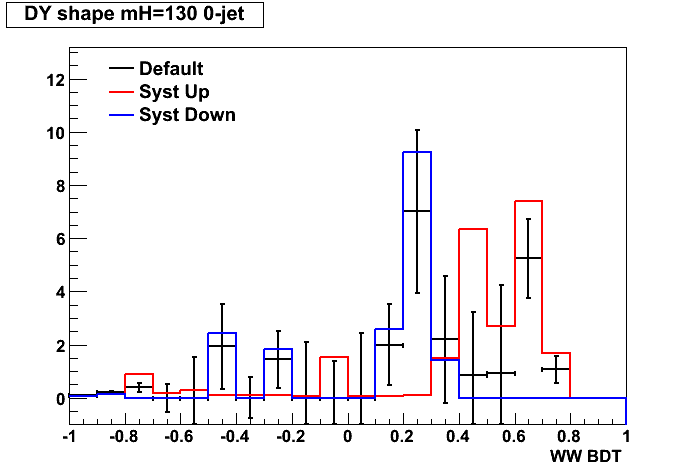
\includegraphics[width=.4\textwidth]{figures/dyshape_zeta/zjets_shape_mh130_0jet.png}}\\
\subfigure[1-jet, \routin~method]{\label{subfig:routin_zjets_shape_mh130_1jet}
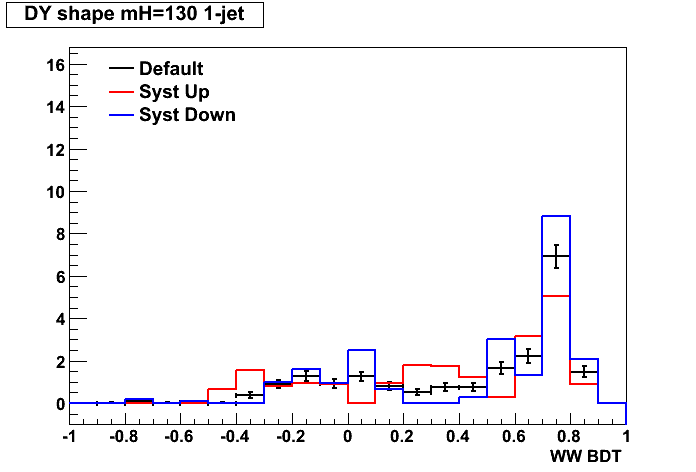
\includegraphics[width=.4\textwidth]{figures/dyshape_routin/zjets_shape_mh130_1jet.png}}
\subfigure[1-jet, \zm~method]{\label{subfig:zeta_zjets_shape_mh130_1jet}
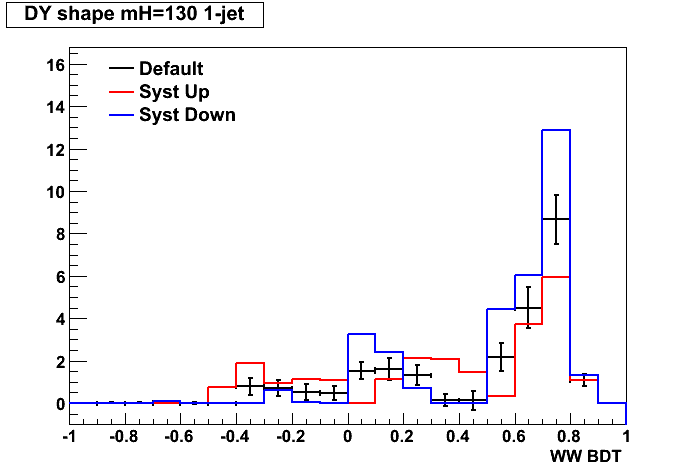
\includegraphics[width=.4\textwidth]{figures/dyshape_zeta/zjets_shape_mh130_1jet.png}}
\caption{\dyll~shape in \mHi=130 \GeVcc analysis.}
\label{fig:zjets_shape_mh130}
\end{center}
\end{figure}
%%%%%%%%

%%%%%%%%
\begin{figure}[!hbtp]
\begin{center}
\subfigure[0-jet, \routin~method]{\label{subfig:routin_zjets_shape_mh140_0jet}
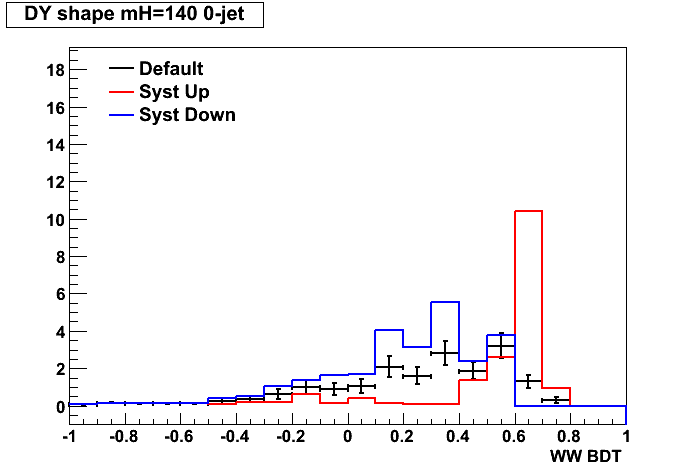
\includegraphics[width=.4\textwidth]{figures/dyshape_routin/zjets_shape_mh140_0jet.png}}
\subfigure[0-jet, \zm~method]{\label{subfig:zeta_zjets_shape_mh140_0jet}
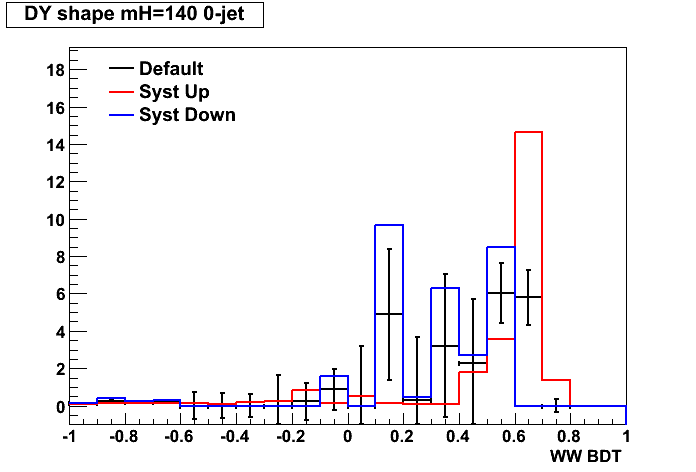
\includegraphics[width=.4\textwidth]{figures/dyshape_zeta/zjets_shape_mh140_0jet.png}}\\
\subfigure[1-jet, \routin~method]{\label{subfig:routin_zjets_shape_mh140_1jet}
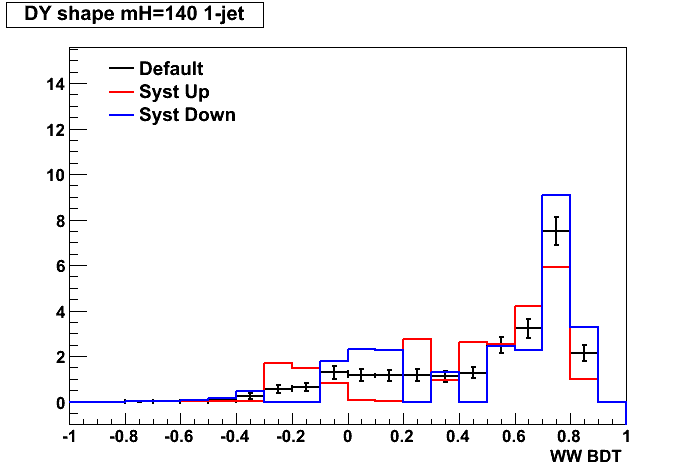
\includegraphics[width=.4\textwidth]{figures/dyshape_routin/zjets_shape_mh140_1jet.png}}
\subfigure[1-jet, \zm~method]{\label{subfig:zeta_zjets_shape_mh140_1jet}
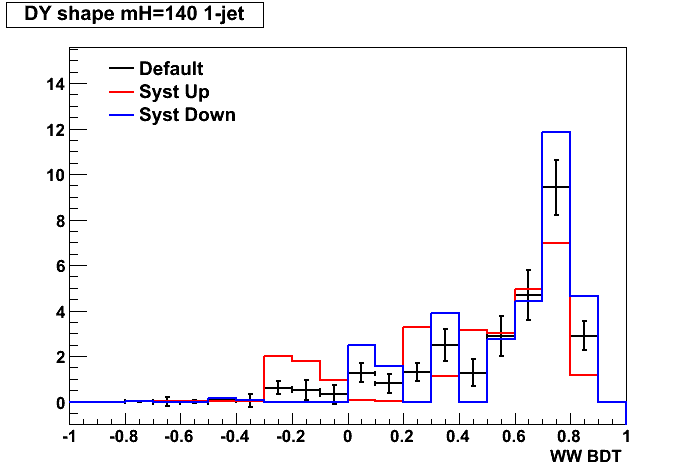
\includegraphics[width=.4\textwidth]{figures/dyshape_zeta/zjets_shape_mh140_1jet.png}}
\caption{\dyll~shape in \mHi=140 \GeVcc analysis.}
\label{fig:zjets_shape_mh140}
\end{center}
\end{figure}
%%%%%%%%

%%%%%
\begin{table}[!ht]
\begin{center}
\begin{tabular} {|c|ccc||ccc|}
\hline
\mHi & Expected & 68\% C.L. & 95\% C.L.  & Expected & 68\% C.L. & 95\% C.L. \\
\hline
\hline
 & \multicolumn{3}{|c||}{\routin, cut based}  & \multicolumn{3}{|c|}{\zm, cut based} \\
\hline
115 & 7.54 & [5.43, 10.49] & [4.05, 14.06]& 6.96 & [5.02, 9.69] & [3.74, 12.99]\\
120 & 4.28 & [3.08, 5.95] & [2.30, 7.98]  & 3.85 & [2.78, 5.36] & [2.07, 7.19] \\
130 & 1.74 & [1.26, 2.43] & [0.94, 3.25]  & 1.59 & [1.14, 2.21] & [0.85, 2.96] \\
140 & 1.04 & [0.75, 1.45] & [0.56, 1.94]  & 0.96 & [0.69, 1.33] & [0.51, 1.79] \\
150 & 0.69 & [0.50, 0.96] & [0.37, 1.29]  & 0.63 & [0.46, 0.88] & [0.34, 1.18] \\
160 & 0.38 & [0.27, 0.52] & [0.20, 0.70]  & 0.36 & [0.26, 0.50] & [0.19, 0.67] \\
170 & 0.38 & [0.27, 0.53] & [0.20, 0.71]  & 0.37 & [0.27, 0.52] & [0.20, 0.70] \\
180 & 0.48 & [0.35, 0.67] & [0.26, 0.90]  & 0.48 & [0.35, 0.67] & [0.26, 0.90] \\
190 & 0.72 & [0.52, 1.01] & [0.39, 1.35]  & 0.72 & [0.52, 1.00] & [0.39, 1.34] \\
200 & 0.91 & [0.66, 1.27] & [0.49, 1.70]  & 0.91 & [0.66, 1.27] & [0.49, 1.70] \\
250 & 2.08 & [1.50, 2.89] & [1.12, 3.88]  & 2.23 & [1.61, 3.11] & [1.20, 4.16] \\
300 & 2.01 & [1.45, 2.80] & [1.08, 3.75]  & 2.38 & [1.71, 3.31] & [1.27, 4.43] \\
\hline
\hline
 & \multicolumn{3}{|c||}{\routin, shape based}  & \multicolumn{3}{|c|}{\zm, shape based} \\
\hline
115 & 6.02 & [4.33, 8.37] & [3.23, 11.22] & 5.66 & [4.07, 7.87] & [3.03, 10.55] \\
120 & 3.12 & [2.25, 4.34] & [1.68, 5.82]  & 3.10 & [2.23, 4.32] & [1.66, 5.79] \\ 
130 & 1.31 & [0.95, 1.83] & [0.71, 2.45]  & 1.52 & [1.10, 2.12] & [0.82, 2.84] \\ 
140 & 0.79 & [0.57, 1.11] & [0.43, 1.48]  & 0.82 & [0.59, 1.15] & [0.44, 1.54] \\ 
150 & 0.57 & [0.41, 0.79] & [0.31, 1.06]  & 0.58 & [0.42, 0.80] & [0.31, 1.08] \\ 
160 & 0.34 & [0.24, 0.47] & [0.18, 0.63]  & 0.30 & [0.22, 0.42] & [0.16, 0.56] \\ 
170 & 0.35 & [0.25, 0.49] & [0.19, 0.65]  & 0.31 & [0.22, 0.43] & [0.17, 0.58] \\ 
180 & 0.44 & [0.31, 0.61] & [0.23, 0.81]  & 0.46 & [0.33, 0.64] & [0.25, 0.85] \\ 
190 & 0.66 & [0.48, 0.92] & [0.36, 1.24]  & 0.69 & [0.49, 0.95] & [0.37, 1.28] \\ 
200 & 0.78 & [0.56, 1.08] & [0.42, 1.45]  & 0.93 & [0.67, 1.30] & [0.50, 1.74] \\ 
250 & 1.75 & [1.26, 2.44] & [0.94, 3.27]  & 2.06 & [1.48, 2.86] & [1.10, 3.84] \\ 
300 & 1.75 & [1.26, 2.43] & [0.94, 3.26]  & 1.85 & [1.33, 2.57] & [0.99, 3.44] \\ 
\hline
\end{tabular}
\caption{Expected limits combining the same flavor final states.}
\label{tab:sf_limits}
\end{center}
\end{table}
%%%%%


%%%%%
\begin{table}[!ht]
\begin{center}
\begin{tabular} {|c|ccc||ccc|}
\hline
\mHi & Expected & 68\% C.L. & 95\% C.L.  & Expected & 68\% C.L. & 95\% C.L. \\
\hline
\hline
 & \multicolumn{3}{|c||}{\routin, cut based}  & \multicolumn{3}{|c|}{\zm, cut based} \\
\hline
115 & 3.26 & [2.35, 4.54] & [1.75, 6.08]  & 3.25 & [2.34, 4.52] & [1.74, 6.06] \\
120 & 2.01 & [1.45, 2.80] & [1.08, 3.75]  & 2.00 & [1.44, 2.79] & [1.07, 3.74] \\
130 & 0.96 & [0.69, 1.33] & [0.51, 1.79]  & 0.95 & [0.69, 1.33] & [0.51, 1.78] \\
140 & 0.62 & [0.45, 0.87] & [0.33, 1.16]  & 0.62 & [0.45, 0.86] & [0.33, 1.15] \\
150 & 0.46 & [0.33, 0.64] & [0.25, 0.86]  & 0.45 & [0.33, 0.63] & [0.24, 0.85] \\
160 & 0.26 & [0.19, 0.36] & [0.14, 0.48]  & 0.26 & [0.18, 0.36] & [0.14, 0.48] \\
170 & 0.27 & [0.19, 0.37] & [0.14, 0.50]  & 0.27 & [0.19, 0.37] & [0.14, 0.50] \\
180 & 0.38 & [0.28, 0.53] & [0.21, 0.71]  & 0.38 & [0.28, 0.53] & [0.21, 0.71] \\
190 & 0.56 & [0.41, 0.78] & [0.30, 1.05]  & 0.56 & [0.40, 0.78] & [0.30, 1.05] \\
200 & 0.70 & [0.50, 0.97] & [0.37, 1.30]  & 0.70 & [0.50, 0.97] & [0.37, 1.30] \\
250 & 1.40 & [1.01, 1.95] & [0.75, 2.61]  & 1.41 & [1.02, 1.96] & [0.76, 2.63] \\
300 & 1.52 & [1.10, 2.12] & [0.82, 2.84]  & 1.57 & [1.13, 2.19] & [0.84, 2.93] \\
\hline
\hline
  & \multicolumn{3}{|c||}{\routin, shape based}  & \multicolumn{3}{|c|}{\zm, shape based} \\
\hline
115 & 2.57 & [1.85, 3.57] & [1.38, 4.79]  & 2.55 & [1.84, 3.55] & [1.37, 4.76] \\
120 & 1.52 & [1.10, 2.12] & [0.82, 2.84]  & 1.52 & [1.10, 2.12] & [0.82, 2.84] \\
130 & 0.70 & [0.50, 0.97] & [0.38, 1.31]  & 0.73 & [0.52, 1.01] & [0.39, 1.35] \\
140 & 0.47 & [0.34, 0.66] & [0.25, 0.88]  & 0.48 & [0.34, 0.66] & [0.26, 0.89] \\
150 & 0.35 & [0.25, 0.49] & [0.19, 0.65]  & 0.35 & [0.25, 0.48] & [0.19, 0.65] \\
160 & 0.22 & [0.16, 0.31] & [0.12, 0.42]  & 0.21 & [0.15, 0.30] & [0.12, 0.40] \\
170 & 0.24 & [0.17, 0.33] & [0.13, 0.45]  & 0.23 & [0.16, 0.32] & [0.12, 0.43] \\
180 & 0.31 & [0.22, 0.43] & [0.17, 0.58]  & 0.31 & [0.23, 0.44] & [0.17, 0.58] \\
190 & 0.45 & [0.32, 0.62] & [0.24, 0.84]  & 0.44 & [0.32, 0.62] & [0.24, 0.83] \\
200 & 0.53 & [0.38, 0.74] & [0.28, 0.99]  & 0.55 & [0.40, 0.76] & [0.29, 1.02] \\
250 & 1.17 & [0.84, 1.63] & [0.63, 2.19]  & 1.21 & [0.87, 1.69] & [0.65, 2.26] \\
300 & 1.27 & [0.91, 1.76] & [0.68, 2.36]  & 1.21 & [0.87, 1.69] & [0.65, 2.26] \\
\hline
\end{tabular}
\caption{Expected limits combining the same flavor and opposite flavor final states.}
\label{tab:sfof_limits}
\end{center}
\end{table}
%%%%%
